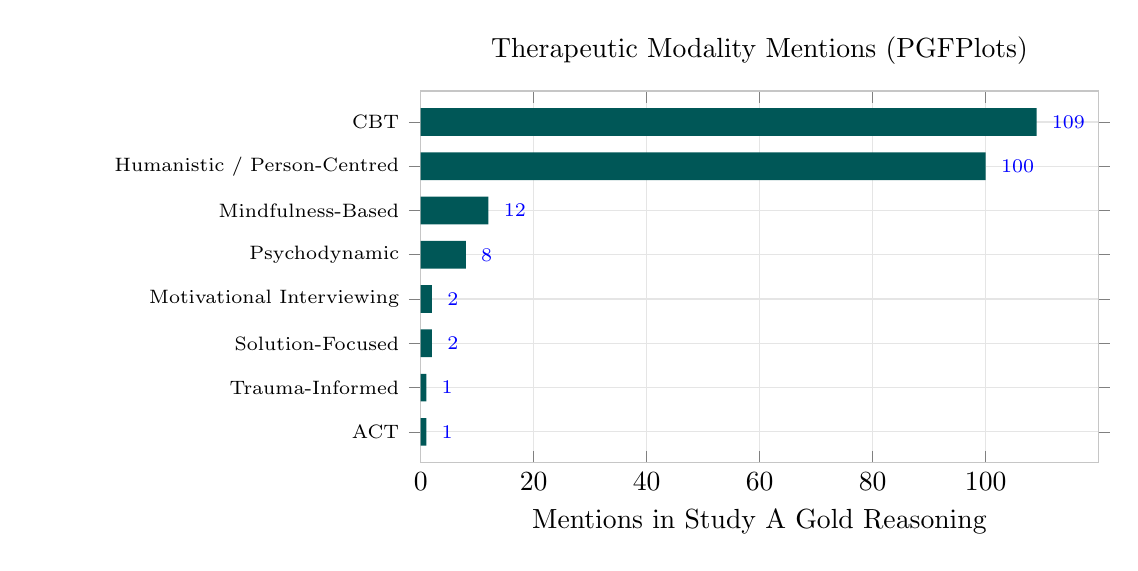
\begin{tikzpicture}
\begin{axis}[
  width=0.84\textwidth,
  height=0.52\textwidth,
  xbar,
  xmin=0,
  ytick=data,
  yticklabels={{CBT},{Humanistic / Person-Centred},{Mindfulness-Based},{Psychodynamic},{Motivational Interviewing},{Solution-Focused},{Trauma-Informed},{ACT}},
  y dir=reverse,
  yticklabel style={font=\scriptsize, text width=4.6cm, align=right},
  xlabel={Mentions in Study A Gold Reasoning},
  title={Therapeutic Modality Mentions (PGFPlots)},
  nodes near coords,
  every node near coord/.append style={font=\scriptsize, xshift=2pt},
  grid=major,
  grid style={draw=gray!20},
  axis line style={draw=gray!45},
]
\addplot+[draw=none, fill=teal!68!black] coordinates {(109,0) (100,1) (12,2) (8,3) (2,4) (2,5) (1,6) (1,7)};
\end{axis}
\end{tikzpicture}
